\chapter{Теоретический раздел}

\section{Работа информационного центра}

\subsection*{Режимы работы}

Всего возможно два режима работы информационного центра. 

\begin{itemize}
	\item Режим нормального обслуживания~---~есть свободные операторы, клиент выбирает свободного оператора с максимальной производительностью.
	\item Режим отказа в обслуживании~---~свободных операторов нет, клиенту отказывается в обслуживании.
\end{itemize}

\subsection*{Переменные имитационной модели}

\begin{itemize}
	\item \textbf{Эндогенные переменные}: время обработки задания $i$-ым оператором, время решения задания $j$-ым компьютером.
	\item \textbf{Экзогенные переменные}: число обслуженных клиентов и число клиентов, получивших отказ
\end{itemize}

\subsection*{Уравнения имитационной модели}

\begin{equation}
	P_{\text{отк}} = \frac{C_{\text{отк}}}{C_{\text{отк}} + C_{\text{обсл}}},
\end{equation}

\noindent где $P_{\text{отк}}$~---~вероятность отказа, $C_{\text{отк}}$~---~количество клиентов, которым отказали в обслуживании, $C_{\text{обсл}}$~---~количество клиентов, которым оказали обслуживание.

\newpage

\subsection*{Структурная схема модели}

\begin{figure}[ht]
    \centering
    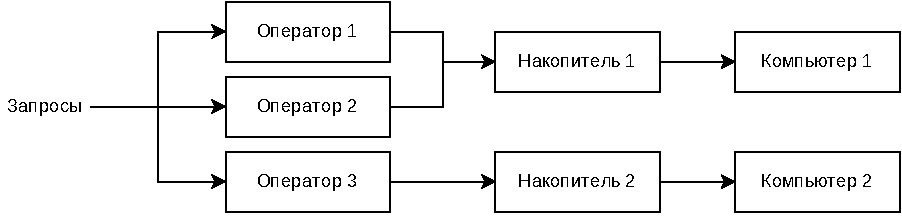
\includegraphics[width=0.8\textwidth]{assets/struct.pdf}
    \caption{Структурная схема модели}
    \label{fig:struct}
\end{figure}

\subsection*{Схема модели в терминах СМО}

\begin{figure}[ht]
    \centering
    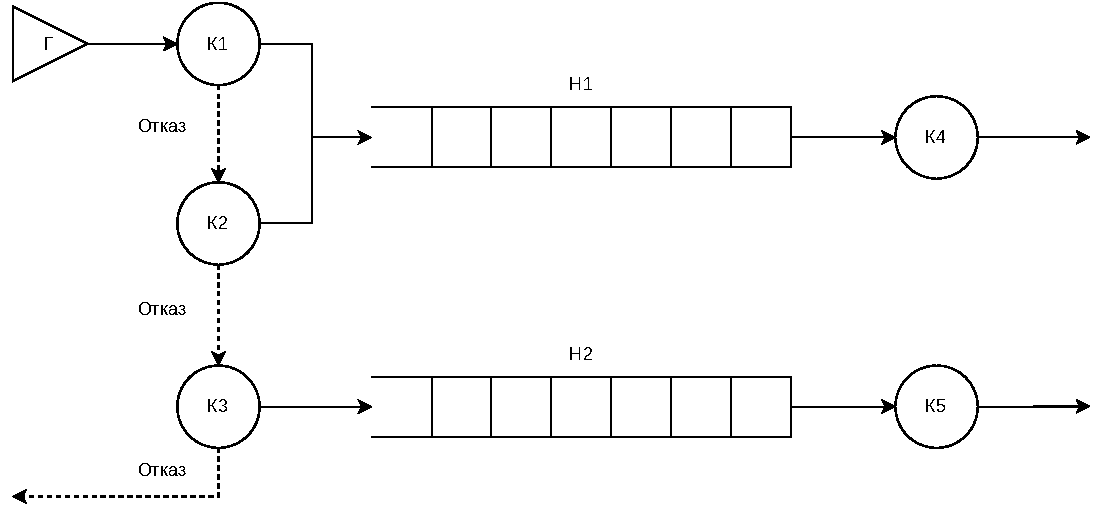
\includegraphics[width=0.8\textwidth]{assets/smo.pdf}
    \caption{Схема модели в терминах СМО}
    \label{fig:smo}
\end{figure}

\section{Событийный алгоритм протяжки времени}

Состояния отдельных устройств изменяется в дискретные моменты времени, совпадающие с моментами поступления сообщений в систему, окончания реализации задания, поэтому моделирование и продвижение текущего времени в системе удобно проводить, используя событийных принцип.

При использовании данного принципа состояние всех блоков имитационной модели анализируется лишь в момент появления какого-либо события.
Момент наступления следующего события определяется минимальными значениями из списка будущих событий, представляющего собой совокупность моментов ближайшего изменения состояний каждого из блоков системы.

